\documentclass[a4paper, 10pt, final, garamond]{book}
\usepackage{cours-preambule}

\titleformat{\item}{}{\arabic{item})}{.5em}{}{}
\titleformat{\subitem}{}{\arabic{item}) \alph{subitem} --}{.5em}
{}{}

\makeatletter
\renewcommand{\@chapapp}{Devoir surveill\'e -- num\'ero}
\makeatother

\begin{document}
\setcounter{chapter}{2}

\chapter{Commentaires sur le DS n\degree3}

\begin{NCprop}[width=\linewidth]{\centering\bfseries\ Rappel des malus}
    Chacune des lettres suivantes sur vos copies sont des malus de \num{1}
    point.\smallbreak
    \begin{minipage}{0.50\linewidth}
        \begin{itemize}
            \item A~: application numérique mal faite~;
            \item N~: numéro de copie incorrect ou manquant~;
            \item P~: prénom sur copies manquant~;
            \item M~: marge non laissée ou trop grande~;
        \end{itemize}
    \end{minipage}
    \begin{minipage}{0.50\linewidth}
        \begin{itemize}
            \item C~: copie grand carreaux~;
            \item U~: unité manquante ou mauvaise~;
            \item H~: homogénéité non respectée~;
            \item $\f$~: loi physique fondamentale brisée.
        \end{itemize}
    \end{minipage}
\end{NCprop}

\begin{brapp}{\includehand{-90}{0.8cm}}
    \begin{center}
        \bfseries Rappel application numérique
    \end{center}
    \begin{minipage}{0.45\linewidth}
        \begin{gather*}
            \boxed{n = \frac{PV}{RT}}
            \qavec
            \left\{
                \begin{array}{rcl}
                    p & = & \SI{1.0e5}{Pa}\\
                    V & = & \SI{1.0e-3}{m^3}\\
                    R & = & \SI{8.314}{J.mol^{-1}.K^{-1}}\\
                    T & = & \SI{300}{K}
                \end{array}
            \right.\\
            \mathrm{A.N.~:}\quad
            \boxed{n = \SI{5.6e-4}{mol}}
        \end{gather*}
    \end{minipage}
    \hfill
    \cancel{\bcancel{
        \begin{minipage}{0.45\linewidth}
            \begin{gather*}
                n = \frac{PV}{RT} = \frac{\num{e5}\cdot\num{1}}{8.32\cdot300}
                = 0.56
            \end{gather*}
        \end{minipage}
    }}
\end{brapp}

\section{Commentaires généraux}

Un assez bon DS, bravo~! Pour refléter cette réussite, la moyenne est à 11/20.
De nettes améliorations de toutes parts et de bonnes surprises. De plus en plus
de copies sans malus, mais des malus encore bêtement acquis. Sur ce DS, au bout
de 3 fois le même malus il est compté double. Malus $\f$ introduit pour les
valeurs temporelles négatives \textbf{qui n'ont pas fait l'objet d'un regard
critique} sur leur négativité, typiquement $\w_0 = -1/\sqrt{LC}$. Il arrive que
des questions rapportent moins de points positifs que de malus~: faites
attention~!

Les rangs ne sont plus indiqués après le premier quartile (12 premières
personnes)~: seul le quartile est indiqué (en noir, encadré). Cf.\ histogramme.

\section{Exercice 1 \hfill \textcolor{red}{/23}}

\begin{enumerate}
    \item Le coefficient stœchiométrique de $\ce{O2}$ est $\frac{25}{2}$. Il
        faut indiquer les états des éléments.
        \hfill \textcolor{ForestGreen}{/2}

    \item \textbf{L'octane liquide n'est \ul{pas un gaz}}~! Environ la moitié de
        la classe a fait cette erreur. Même si on ne l'utilise pas, la colonne
        $n_{\tot, gaz}$ était attendue. Ceci dit, 1 seule personne a
        correctement rempli la quantité de gaz~: $n_{\ce{O2}} + n_{\ce{N2}}$.
        \textbf{Faites attention à qui est un gaz dans ce décompte}. De même,
        attention aux applications numériques, et \textbf{aux unités de la loi
        du gaz parfait}~! Points pour \textbf{citer la loi de Dalton}. Mais le
        plus important~: ça n'est pas le \textbf{\ul{volume}} de dioxygène qui
        est 1/5 du volume de l'air, c'est sa \textbf{\ul{quantité de matière/sa
        pression}}~!
        \hfill \textcolor{ForestGreen}{/15}

    \item Très bonnes réponses là-dessus, de très bonnes recherches et
        compréhension de la question. Différentes approches récompensées de la
        même manière, la méthode du corrigé n'est pas la seule manière d'y parvenir.
        \hfill \textcolor{ForestGreen}{/6}
\end{enumerate}

\section{Problème 1\hfill \textcolor{red}{/42}}

\begin{enumerate}
    \item Cette force est celle de \textbf{frottements fluides} (ou visqueux).
        Ça n'est pas la force du ressort (ou le poids). On demandait \textbf{le
        signe de $\lambda$}, pas le signe \cancel{devant} $\lambda$~: la
        constante est positive et s'oppose au \ul{déplacement}.
        \hfill \textcolor{ForestGreen}{/3}

    \item Il faut établir le \textbf{système} et le \textbf{référentiel}, faire
        un \textbf{schéma}, un clair et détaillé \textbf{bilan des forces},
        énoncer la deuxième loi de \textsc{Newton} (ou PFD) et être cohérent-e
        dans les grandeurs~: $x$ n'est pas $z$~! Peu de rigueur ici.
        \hfill \textcolor{ForestGreen}{/9}

    \item La \textbf{pulsation} n'est pas la \textbf{fréquence}. Attention à
        l'homogénéité de vos formules.
        \hfill \textcolor{ForestGreen}{/4}

    \item Il faut savoir résoudre~: équation caractéristique, déterminant, signe
        du déterminant, racines de l'équation caractéristique, définition de
        $\w$ et forme de la solution.
        \hfill \textcolor{ForestGreen}{/6}

    \item Pulsation $\neq$ fréquence. Attention aux unités.
        \hfill \textcolor{ForestGreen}{/2}

    \item Que deux estimations de $Q$ dans les 46. Différentes approches
        possibles~: $t_{95}$ ou $5\tau$.
        \hfill \textcolor{ForestGreen}{/4}

    \item \textbf{Les frottements modifient la fréquence}~: $\w = \w_0 \sqrt{1 -
        \frac{1}{4Q^2}}$. Il fallait voir si $\w \approx \w_0$.
        \hfill \textcolor{ForestGreen}{/4}

    \item 1 seule exploitation des deux documents sur les 46. Il faut savoir
        exploiter les graphiques.
        \hfill \textcolor{ForestGreen}{/10}
\end{enumerate}

\section{Problème 2\hfill \textcolor{red}{/58}}

\begin{enumerate}
    \item Il faut le schéma avant fermeture~: c'est lui qui définit la charge du
        condensateur. \textbf{On voulait justifier que sa tension chargée était
        $E$}~: interrupteur ouvert, loi des mailles. Attention à l'homogénéité~:
        $q \propto CE$, pas $E$, pas $E/C$.
        \hfill \textcolor{ForestGreen}{/4}

    \item Question super bien réussie~!
        \hfill \textcolor{ForestGreen}{/6}

    \item On peut admettre la forme $A\cos + B\sin$, mais si vous voulez la
        démontrer avec l'équation caractéristique et les racines complexes
        (ce qui est super, retenez le moins de choses possibles) prenez bien
        $\Ir = \sqrt{-1}$ pour éviter de tomber sur des solutions
        exponentielles. Très peu de justification des conditions initiales.
        \textbf{Il faut savoir résoudre}~! Savoir-faire $\gg$ savoir.
        \hfill \textcolor{ForestGreen}{/3}

    \item Les formes $W_L$ et $W_C$ ($\mathcal{E}_C$ et $\mathcal{E}_L$) sont
        considérées connues. Plein de points à aller chercher ici.
        \hfill \textcolor{ForestGreen}{/10}

    \item \textbf{Oscilloscope}, pas oscillateur.
        \hfill \textcolor{ForestGreen}{/1}

    \item Question très bien réussie aussi~! Pensez à refaire le schéma.
        \hfill \textcolor{ForestGreen}{/7}

    \item RAS
        \hfill \textcolor{ForestGreen}{/5}

    \item 
        \begin{enumerate}
            \item Simple application numérique, mais \textbf{il faut connaître
                l'unité d'une pulsation} et éviter d'avoir une réponse fausse +
                un malus.
                \hfill \textcolor{ForestGreen}{/1}
            \item RAS
                \hfill \textcolor{ForestGreen}{/8}
        \end{enumerate}
    \item Revoyez l'impact du facteur de qualité. $Q \ll 1 \Rightarrow$ régime
        \textbf{apériodique}. Attention aux conditions initiales~: tangente à
        l'origine nulle. Plein de points à prendre sur cette question
        «~connaissances physiques~».
        \hfill \textcolor{ForestGreen}{/7}
\end{enumerate}

\section{Problème 3\hfill \textcolor{red}{/52}}

\begin{enumerate}
    \item Si vous calculez un $K\degree$, il faut commenter l'avancement~: total
        ou négligeable. Pensez à $n_{\tot, gaz}$.
        \hfill \textcolor{ForestGreen}{/6}
    \item Citez la \textbf{loi d'action des masses} ($K\degree = Q_{r, \eq}$).
        Détaillez vos calculs~: 1 point pour l'activité, pour la simplification,
        pour la loi de \textsc{Dalton}, la fraction molaire…
        \hfill \textcolor{ForestGreen}{/6}
    \item Pas mal pour qui l'a fait. Approche avec $K\degree+1$ dans les calculs
        préférée (mais approche du corrigé ok).
        \hfill \textcolor{ForestGreen}{/8}
    \item RAS
        \hfill \textcolor{ForestGreen}{/3}
    \item RAS
        \hfill \textcolor{ForestGreen}{/3}
    \item Autre polynôme second degré, très bonne récompense en points mais très
        peu traitée.
        \hfill \textcolor{ForestGreen}{/10}
    \item Pas mal.
        \hfill \textcolor{ForestGreen}{/6}
    \item Autre (autre) polynôme second degré, très bonne récompense en points
        mais très peu traitée.
        \hfill \textcolor{ForestGreen}{/10}
\end{enumerate}

\vfill

\begin{center}
    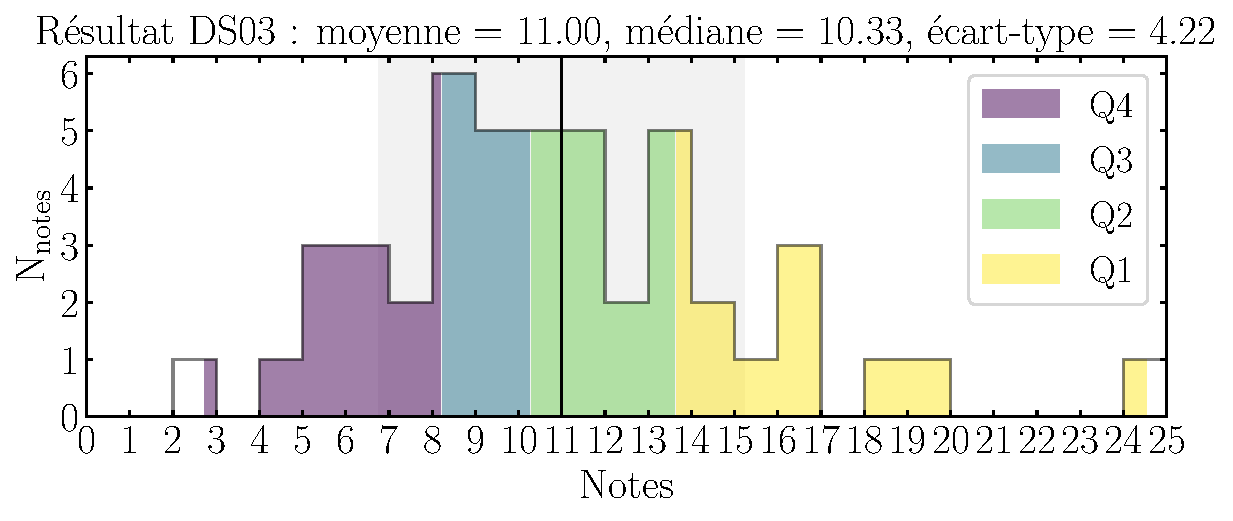
\includegraphics[width=.72\linewidth]{res_DS03.pdf}
\end{center}

\vfill

\end{document}
